\begin{frame}{вывод формулы}
\begin{equation}
p^{'}=\frac{8T^{'}}{3\left(\n\upsilon'-1/3\right)}-\frac{3}{\left(\upsilon'\right)^2},
\label{eq:1}
\end{equation}
\[ \quad   p^{'}=\frac{p}{p_{c}},\ \quad \quad \upsilon^{'}=\frac{\upsilon}{\upsilon_{c}},\quad \quad T^{'}=\frac{T}{T_{c}}\]
\(p,\upsilon \ and \ T\) - давление, объём и температура, соотвественно,нижний индекс 'с' относится к критическим значениям, а простое число к приведённым координатам. Точка максимального перегрева \(T_{M^{'}}\) находим из уравнения: 
\vspace{0.25cm}\({\left(\frac{\partial p^{'}}{\partial \upsilon^{'}}\right)}_{T^{'}}=0\), откуда: \ \(\frac{8T_{M^{'}}}{3{\left(\upsilon_{M^{'}}-\frac{1}{3}\right)}^{2}}=\frac{6}{{\upsilon_{M^{'}}}^{3}}\),\  подставим полученное
\vspace{0.25cm}
выражение в (\ref{eq:1}) , получим: \(p_{M^{'}}=\frac{1}{\left({\upsilon_{M^{'}}}\right)^{2}}\left[\frac{2\left(3{\upsilon_{M^{'}}-1}\right)}{{\upsilon_{M^{'}}}}-3\right]\)
\end{frame}
\begin{frame}{продолжение}
 объеденим вышеуказанные уравнения, чтобы получить \(T_{M^{'}}\) как функцию от \(p_{M^{'}}\). Напрример, если \(p_{M^{'}}=0\), то \(T_{M^{'}}=\frac{27}{32}T_{c}\), все эти выкладки справедливы в пределах нормально атмосферного давления.
\center{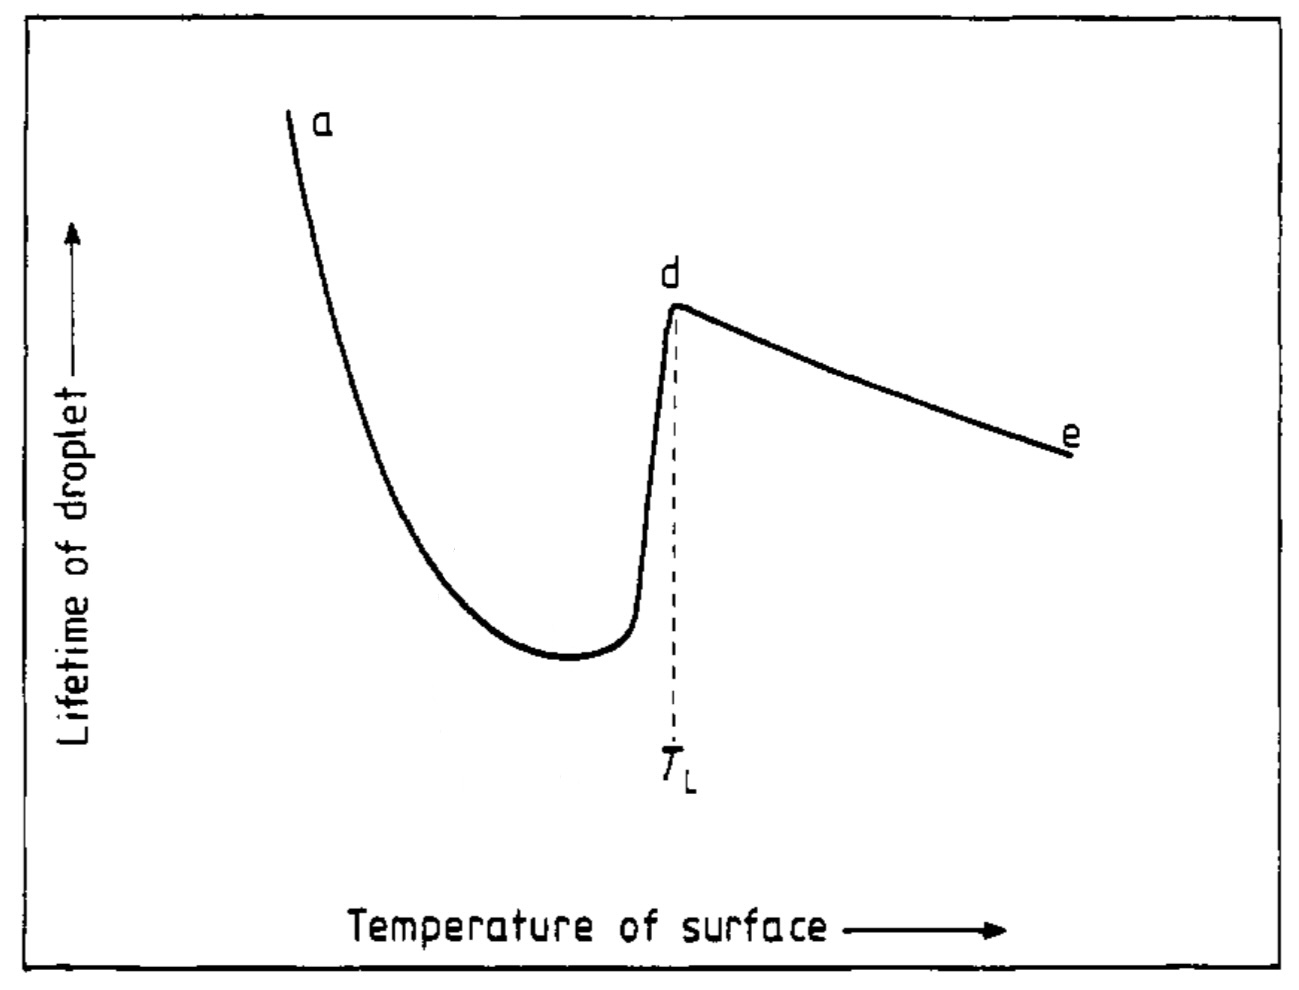
\includegraphics[scale = 0.14]{IMG_7600.jpg}}
\end{frame}
